\documentclass[a4paper,12pt]{article}

\usepackage{graphicx}
\usepackage{amsmath}
\usepackage{hyperref}
\usepackage{fancyhdr}

\renewcommand{\abstractname}{Summary}

\title{D.I.A.G.R.A.M.: Development of Image Analysis for Graph Recognition And Modeling}
\author{Filippo Garagnani, Saverio Napolitano, Nicola Ricciardi}
\date{\today}

\pagestyle{fancy}
\fancyhead[L]{D.I.A.G.R.A.M. - Project Proposal}
\fancyhead[R]{\small Garagnani, Napolitano, Ricciardi}

\begin{document}

\maketitle

\begin{abstract}
    This project proposes the development of a system for analyzing different types of handwritten diagrams and converting them into well-rendered images through a textual syntax. The goal is to create a tool capable of analyzing scanned or photographed sketches of diagrams and automatically generating code that can be rendered into the same diagrams digitally, to eventually integrate or modify them.
\end{abstract}

\section{Introduction}
    Diagrams are a powerful means of representing complex systems, ideas, and relationships. Writing diagrams in a textual format is extremely efficient to easily edit the diagram and to display it in a better-formed format. This project aims to automate the conversion of handwritten diagrams into code, streamlining the process of diagram creation and visualization.

\section{Objective}
    The main objective of the D.I.A.G.R.A.M. system is to:
    \begin{itemize}
        \item Develop a computer vision model to recognize handwritten diagrams.
        \item Extract relevant features from the diagrams (nodes, edges, labels).
        \item Generate equivalent code in supported languages for the recognized diagrams.
        \item Automatically parse the code to generate the formatted image of the input diagram.
    \end{itemize}
    
\section{System Architecture}
    The project will be composed of different modules that will be stacked together in an uniform pipeline [\textbf{Figure 1}]. These components are:
    \begin{itemize}
    		\item \textbf{Preprocessor}: Applies some operations (like denoising, rotation...) in order to obtain a more suitable input image for the following modules.
    		\item \textbf{Classifier}: In order to manage more than one type of diagrams, a classifier that identifies the category of the input diagram is needed.
    		\item \textbf{Extractor}: By employing feature extraction, image segmentation and static analysis over the recognized components, the extractor will output a robust structure to contain all the relevant information about the diagram. This key component takes the image as input and will output the entities found, their relations and more useful information.
    		\item \textbf{Transducer}: From the data output by the extractor, a certain transducer will give out a formatted code relative to the input diagram. We envision a single transducer for every supported language.
    		\item \textbf{Compiler}: Given the code, the compiler will convert it into an output image - hopefully, as close as possible as the input diagram.
    \end{itemize}

\begin{figure}[h]
    \centering
    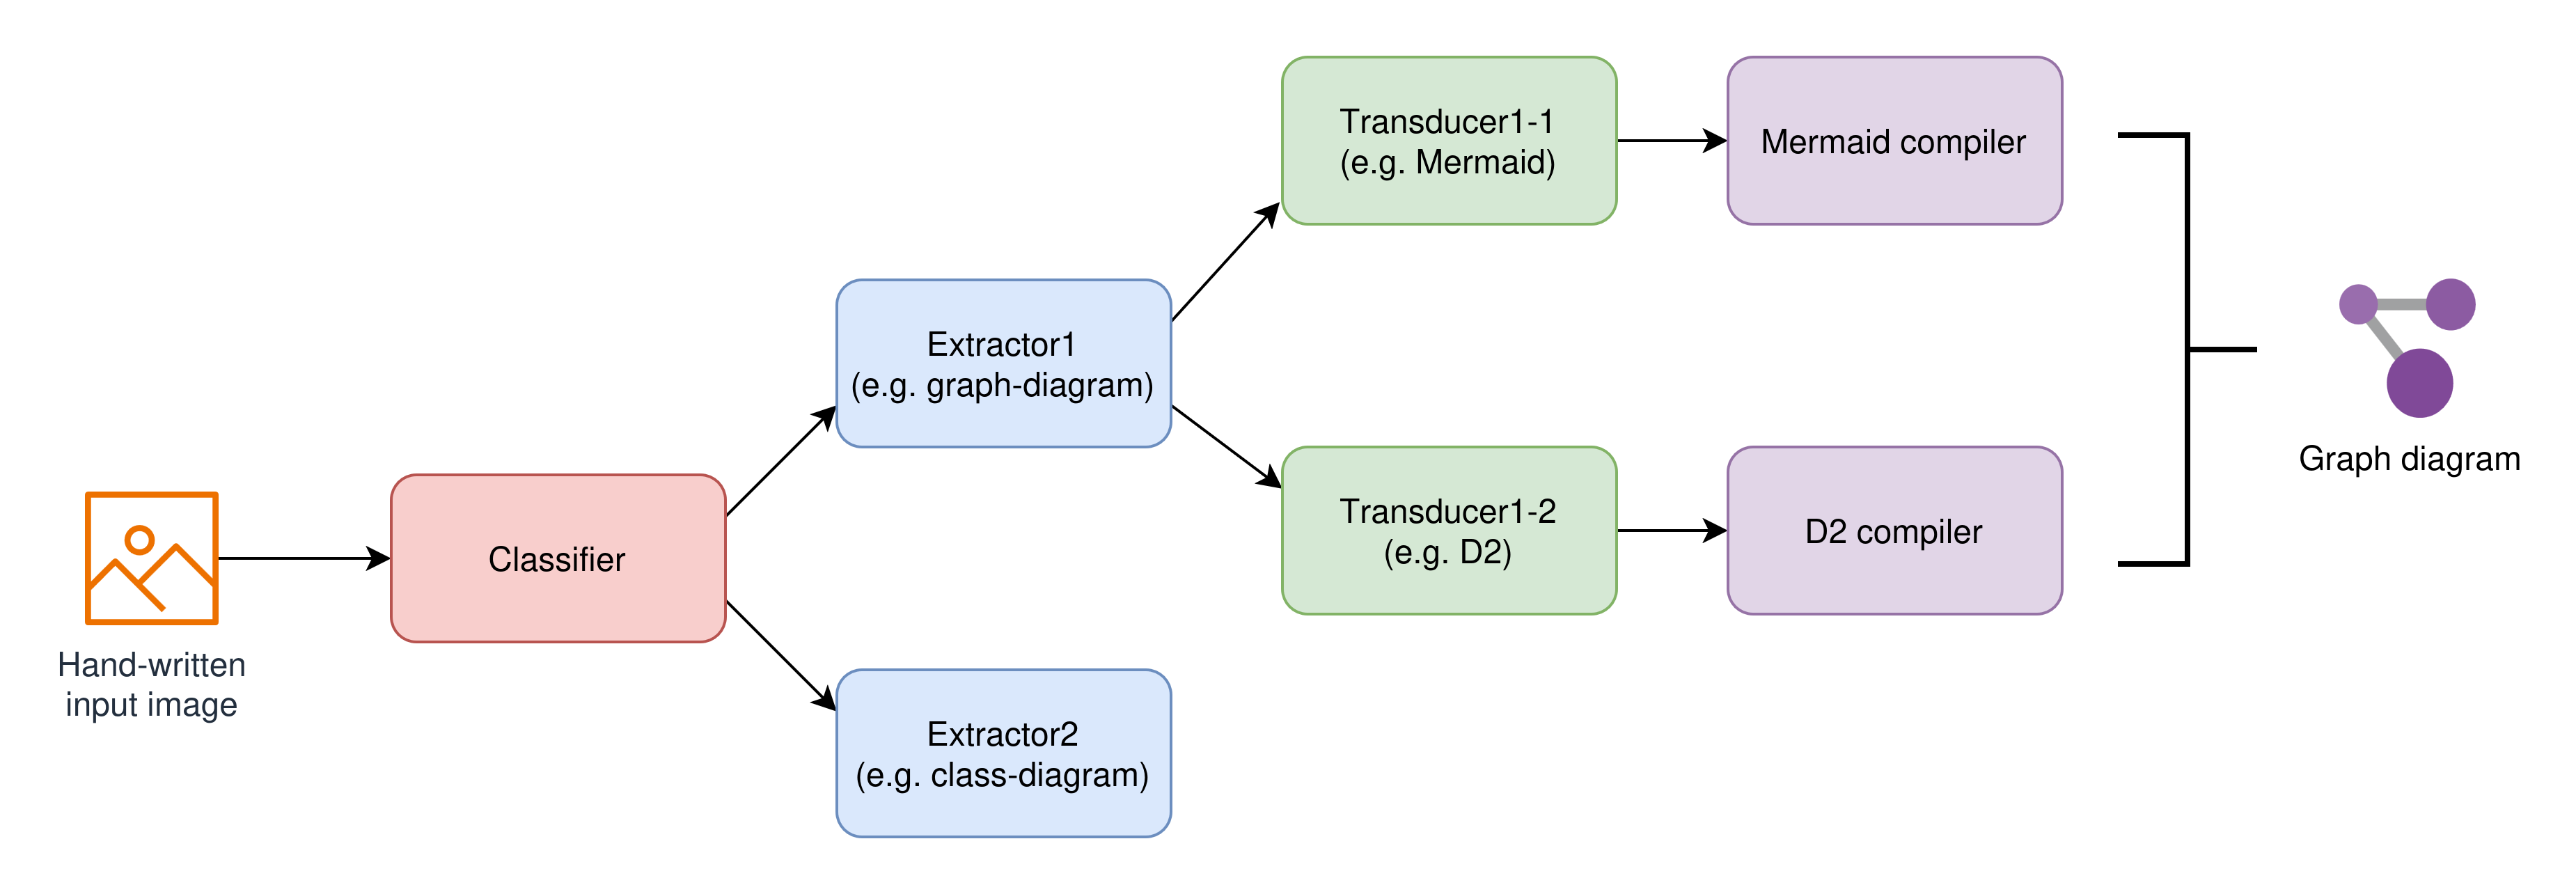
\includegraphics[width=1.2\textwidth]{../assets/images/overview.png} % Change the path to your image
    \caption{The D.I.A.G.R.A.M. pipeline.}
\end{figure}

\newpage

\section{Constraint}
While the whole project idea could be applied to a wide variety of diagrams and languages, in order to manage the complexity we decided to impose a few theoretical constraints:

	\begin{enumerate}
	
	\item \textbf{Types of diagrams}: We restrict the types of diagrams that the system is able to correctly recognize and reconstruct (\textit{e.g.} Graph diagrams, Flowchart diagrams...)
	\item \textbf{Languages}: Even if there are various languages in which the diagrams could be formatted, we limit the languages that the system could translate the diagrams to (\textit{e.g.} Mermaid, D2...)
	
	\end{enumerate}

\end{document}
